\documentclass[a4paper]{article}

%% Language and font encodings
\usepackage[english]{babel}
\usepackage[utf8x]{inputenc}
\usepackage[T1]{fontenc}

%% Sets page size and margins
\usepackage[a4paper,top=3cm,bottom=2cm,left=3cm,right=3cm,marginparwidth=1.75cm]{geometry}

%% Useful packages
\usepackage{amsmath}
\usepackage{graphicx}
\usepackage[colorinlistoftodos]{todonotes}
\usepackage[colorlinks=true, allcolors=blue]{hyperref}
\usepackage{subfigure}
\usepackage{caption}
\usepackage{amsfonts}
\usepackage{amsthm}
\usepackage{upquote}
\usepackage{listings}
\usepackage{enumitem}
\usepackage{dirtytalk}
\usepackage{hyperref}
\usepackage{float}

\def\therefore{\boldsymbol{\text{ }
\leavevmode
\lower0.4ex\hbox{$\cdot$}
\kern-.5em\raise0.7ex\hbox{$\cdot$}
\kern-0.55em\lower0.4ex\hbox{$\cdot$}
\thinspace\text{ }}}

\title{Generating lecture notes out of a lecture video}
\author{CSED Sung Haebin 20160463}

\begin{document}
\maketitle
\section{Summary}
This project is about generating lecture notes out of a lecture video.
The goal is to recover images of a board scene, recovering the parts of the board that the lecturer occluded.

\section{Motivation}
Sometimes, when you watch a lecture video, it is painful to write lecture notes. 
If we automatically generate lecture notes, then it would definitely be convenient.

\section{Goals}
\subsection{Board Detection and Extracting Human Pixel}
We first have to know where the board is, to generate a picture of the board. Even if the camera is not looking at the board orthogonally, it's no problem, because we could calculate the homography matrix since we know that the board is rectangular. Then we have to extract the human(lecturer) part of a board to get rid of it. The most essential part of this project is to know whether a human is blocking the board or not, since we want to get rid of the human pixel.
\subsection{Board Transition Detection}
When do we have to take a snapshot? I would guess when it's when a lecturer erases the board, or when it moves to a new board, or when the board changes. I call this as a 'board transition'. This part is the most hardest part, because every lecture has different transitions with different magnitude, and it's hard to catch them all. For example, what if the lecturer erases only part of the board, and keeps going on? It is quite a task to detect them significantly.
\subsection{Board Recovery}
We now know the timing when we need to extract board images, so we recover the board in that time interval. We need to use a scheme to effectively predict 
\subsection{(Optional) Making images to a pdf file}
A lecture note is best if it exists as a pdf, since a bunch of images are rather uncomfortable to keep.

\section{Implementation}
\subsection{Development Environment and Dataset}
In this project we need direct controlling of the shaders, especially fragment shaders.
Or even there could be some arbitrary change of pipeline in overall, because extreme features of fractal geometry could require some modification of typical graphics procedures.
And also one of our goal is about optimization of this particular task, so we consider low-level programming.

And fractals are not highly related to photo realism, so many pre-developed presets and modules provided by
graphics engines such as Unity won't be particularly helpful.
Thus we'll develop this project with pure OpenGL(with glut, glm, ...)
\subsection{Human Exclusion by Semantic Segmentation}
The key idea of rendering fractals is using fragment shaders wisely.
'Escape-time fractals', such as Mandelbrot set is rendered based on the speed of diversion for every complex coordinates.
So those kinds of fractals will require the renderer to perform per-pixel calculation, which is the reason fragment shaders are for.

And vertex shaders are also important.
To construct 3D space of fractals, we should choose either voxel rendering or 3D polygons with 2D fractal textures.
Voxel is very intutive and expressive, but needs an enormous amount of calculation.
Thus we consider 3D polygons, but those polygons should be also complex and fractalistic enough.
We also expect an animation of fractal space, so vertex shaders also must be used well.
\subsection{Advanced Rendering Techniques}
Advanced techniques like shading, texture, arbitrary clipping, aliasing would make the final quality better or even produce some novel graphic.
Our lecture hasn't covered those topics yet, so we will think about this later.

\subsection{scheme}
If we want to render fractals in real time, optimization will be important.
Here are some schemes we've thought about.

\textbf{Parallel Processing}
Yes, of course shaders are exactly for parallel procesing.
We will exploit the benefits of using parallel programming as much as we can, trying to put many works on shaders.
Or even cpu may need to be parallized.

\textbf{Cache}
Some fractals may have symmetric features or repeated geometry (for strict fractals).
Instead of just re-calculating those parts, we can keep them and reuse.
If the data we want to keep is result of shaders, then we need to think about whether saving some calculated data in gpu is possible and eventhough, if it is efficient.

\textbf{Dynamic Resolution}
Rendering fractals in high resolution will be necessary, but not for everywhere.
If the polygon we want to render fractal on is too far or too tilted, then we can consider lowering resolution for only that place.
(Remember that what we try to do is rendering fractals \textit{on polygons})

\textbf{Keeping the buffer}
We can reuse some part of frame buffer for last scene, which is not common.


\section{Notable References}
\subsection{Deeplabv3}
\url{https://arxiv.org/abs/1706.05587}
There are 3 reference textbooks we'll study.
\textit{Interactive Computer Graphics}\cite{c1}, our course textbook, introduces some background of fractal geometry and examples like Mandelbrot Set.
\textit{OpenGL SuperBible}\cite{c2} introduces rendering methods of Julia fractals using shader.
\textit{Rendering Methods for 3D Fractals}\cite{c3} introduces volume rendering methods for fractal rendering and methods for 3D Fractal high resolution image. We can choose techniques for 3D fractal calculation and rendering.

\subsection{Fragmentarium}
\textbf{Fragmentarium} is an open source, pixel-based graphics rendering tool, which is part of what we want to do.
The program's input script is based on GLSL, with some added functionalities and preprocessors.
Fragmentarium is good for generating fractal art, such as \url{https://www.flickr.com/groups/fragmentarium/}.
It is open source and based on GLSL shaders, so we think we could get something out of it.
You could get more details from \url{http://syntopia.github.io/Fragmentarium/index.html}.

\section{Gallery}
\begin{figure}[H]
\centering
\subfigure[scene from a Youtube video(\url{https://youtu.be/S530Vwa33G0})]
{
    \label{fig:subfig1}
    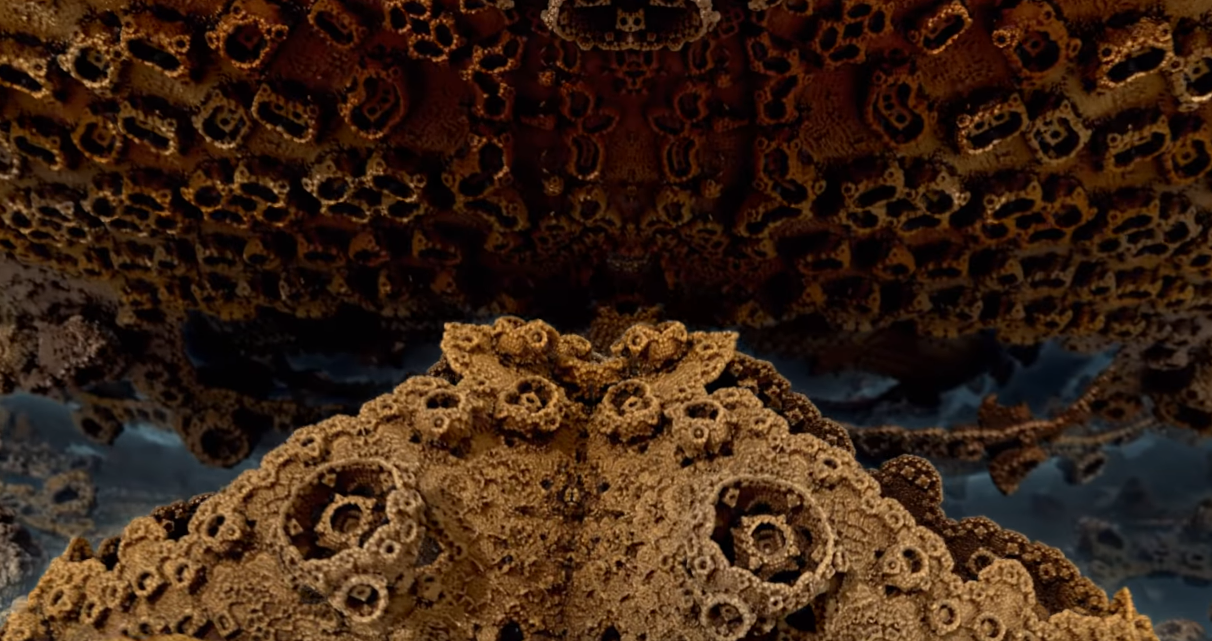
\includegraphics[scale=0.3]{cap1.PNG}
}
\end{figure}

\begin{figure}[H]
\centering
\subfigure[a Mandelbrot Set(\url{https://en.wikipedia.org/wiki/Mandelbrot_set})]
{
    \label{fig:subfig2}
    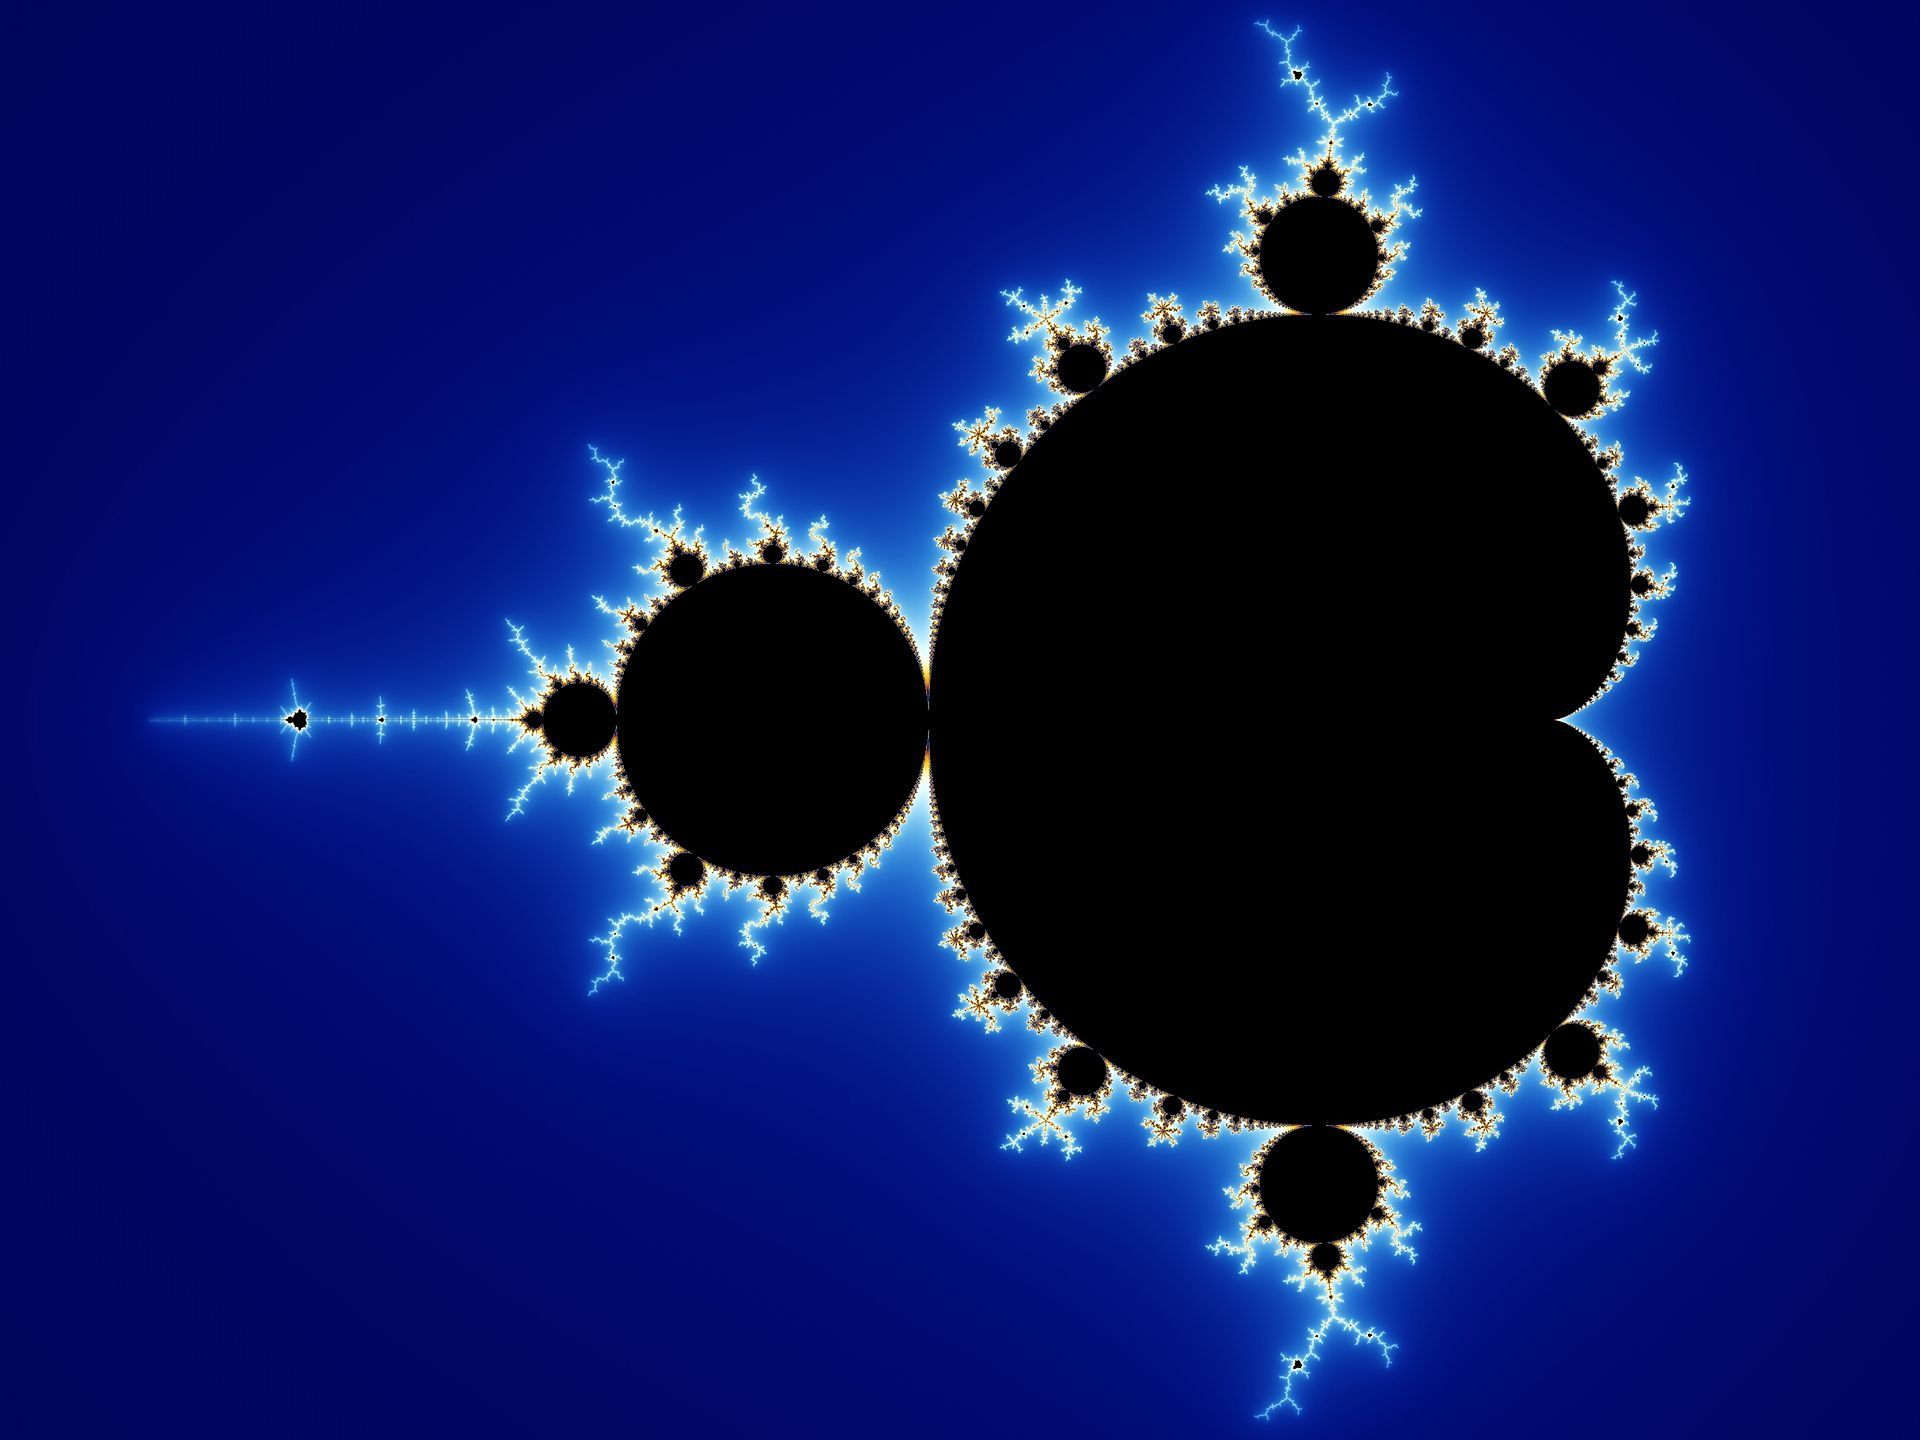
\includegraphics[scale=0.3]{mandel.jpg}
}
\end{figure}
\section{Discussion}
There are some issues in this project.
\begin{description}[style=nextline]
\item[Is rendering such high resolution 3D fractals possible in realtime?]
We agree that it's difficult generally, so some loss of quality could be inevitable.
But we believe most of the overhead can be optimized using very specialized techniques with a well-developed program.
\item[What level of achievement do we expect?]
Studying, researching and implementing all those features mentioned will be our goal.
The quality of product that we desire is slightly less than common fractal videos in Youtube, because we're doing in realtime. (search \say{3D fractal})
\item[What are our roles?]
Not clearly separated, but we have some background knowledge. Junha has exeperienced fractals before and familiar with machine learning. (Not sure if it is useful)
Sangwoo knows how to deal with videos(PBS). Haebin is good at low-level and system programming.
\end{description}

\begin{thebibliography}{1}
\bibitem{c1}E. Angel and D. Shreiner, Interactive Computer Graphics: A Top-Down Approach with Shader-Based OpenGL, 6th ed., Addison-Wesley, 2011, p.487 Section 9.8 Recursive Methods and fractals
\bibitem{c2}Graham Sellers; Richard S. Wright, Jr.; Nicholas Hanemel, OpenGL SuperBible, 7th ed., Addison-Wesley, p.683 Rendering Julia Fractals
\bibitem{c3}Rickard Englund, Rendering Methods for 3D Fractals
\textit{Science and Engineering Ethincs}, 2009, pp. 311-341.
\end{thebibliography}

\end{document}
